\section{Base de datos de artículos}
Para comprender el comportamiento de los resultados de las búsquedas se diseñaron dos tipos de gráficos con la intención de es visualizar los resultados que tan cohesivos son los bundles y la distancia que existe entre estos. De esta forma se podrá analizar la calidad del resultado obtenido más allá del valor de la función objetivo.\\
En los gráficos de \ref{res:img-explain-bars} se visualiza a través del tamaño de un círculo la proporción de cada artículo con cada tópico y con el color del artículo al bundle al que pertenece. Por lo tanto si para un bundle se tiene que la distribución entre los tópicos y el tamaño de los círculos es similar para cada artículo se puede deducir que ese bundle es cohesivo. Por otro lado si los círculos de un bundle no coinciden con los círculos de otro bundle el resultado es diverso.
\begin{figure}[H]
  \centering
    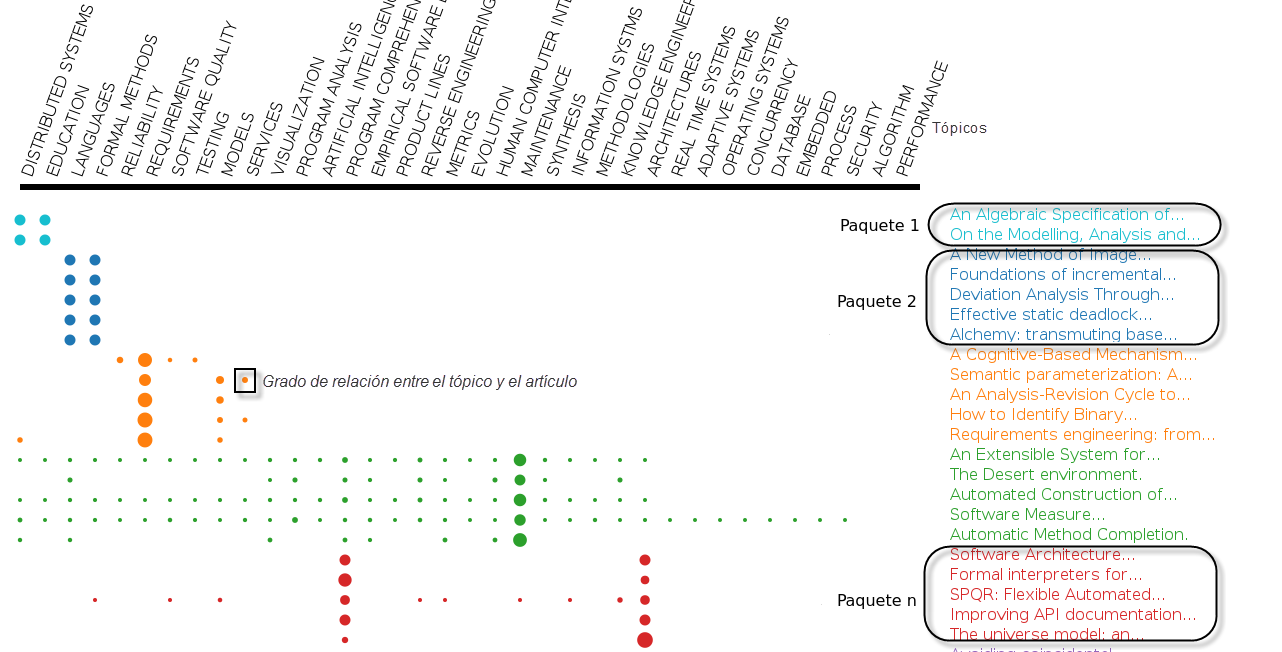
\includegraphics[width=1\textwidth]{img/explain-bars.png}
  \caption{}
  \label{res:img-explain-bars}
\end{figure}

En los gráficos de tipo burbuja \ref{res:img-explain-bubbles} se observa la relación entre los tópicos y los bundles. Cada burbuja representa un tópico y contiene los círculos de la proporción en la relación entre el tópico que representa y un artículo del resultado, además el color del círculo representa al bundle al que pertence el artículo. Entonces si las burbujas contienen círculos de más de un color se puede decir que ese resultado no es muy diverso, mientras que el color de los círculos de las burbujas sea más homogéneo el resultado es más diverso. En cuanto a la cohesión de los bundles, es más cohesivo cuando el tamaño de cada circulo dentro de cada burbuja sea similar (para el mismo color) y la distribución de los círculos entre cada burbuja es equitativa.

\begin{figure}[H]
  \centering
    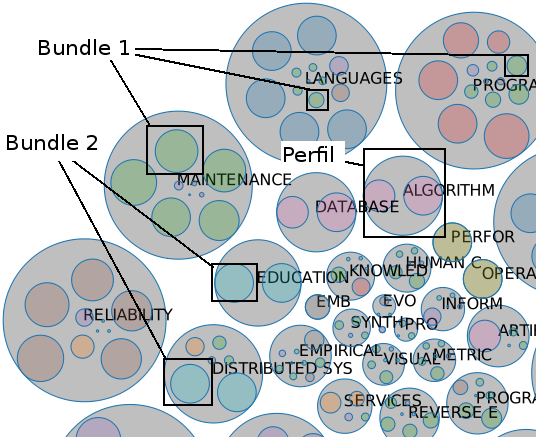
\includegraphics[width=0.5\textwidth]{img/explain-bubbles.png}
  \caption{}
  \label{res:img-explain-bubbles}
\end{figure}
\subsection{Búsquedas de Artículos}\label{res:busPaper}
Generar una solución, en el que cada bundle contenga artículos similares que se hayan presentado en distintas conferencias.\\
\begin{itemize}
  \item \textbf{Similitud}: Función que compara el perfil de cada artículo.
  \item \textbf{Complementariedad}: Lugar dónde fue presentado.
\end{itemize}

La base de datos de \cite{dataDrive} contiene $7777$ artículos, para las búsquedas se requiere que cuenten con la información del autor, de los tópicos (\textbf{topic profile}) y el lugar de publicación (\textbf{venue}). Los artículos que no cuentan con alguno de estos datos no se tuvieron en cuenta para la experimentación. A partir de las primeras ejecuciones y resultados obtenidos se observaron dos comportamientos no deseados, \textit{soluciones similares para distintos valores de $\gamma$} y \textit{soluciones con bundles unitarios}, a continuación se explica con más detalle estos comportamientos.\\
Al finalizar la depuración de artículos que se consideró afectaban los resultados obtenidos, se obtuvieron $3954$ para realizar todas las pruebas mencionadas.
\paragraph{Soluciones similares para distintos gammas}
En las primeras ejecuciones realizada se observa que el valor de la función objetivo se encuentra cercano a una cota máxima (ver \ref{conc:valoresOptimos}) y que para todos los valores de $\gamma$ utilizados las soluciones eran muy similares entre sí. Realizando un análisis más detallado sobre los resultados se detectó que la mayoría de los bundles contenían artículos de un solo tópico, por los bundles son muy cohesivo (alto valor \textbf{intra}) y muy diversos entre si (alto valor \textbf{inter}).\\
Al contar con muchos artículos con un solo tópico las soluciones obtenidas no permiten realizar una correcta comparación de las heurísticas, por lo tanto a fines prácticos de comparar las distintas implementaciones y obtener un conjunto de bundles más interesantes, se decidió eliminar los artículos que contengan un solo un tópico.
\paragraph{Soluciones con bundles unitarios}
Las soluciones obtenidas mediante las búsquedas en las que se prioriza que los bundles sean más cohesivos (\textbf{inter}) contenían una alta cantidad de bundles con uno o dos elementos únicamente, tal conducta no es la deseada ya que queda una parte del presupuesto sin ser usado.\\
Este comportamiento ocurre particularmente con el método jerárquico o HAC en la etapa de producción del algoritmo \texttt{PAC}, ya que algunos cluster generados no superan el presupuesto pero no pueden ser unidos con otro cluster porque invalida la complementaridad que se quiere lograr. Suponiendo que para la búsqueda \textit{Artículos de diferentes conferencias} existen los artículos $A_1$, $A_2$, $A_3$, $A_4$ y $A_5$ y tienen una distribución del tópico $t$ mayor a $0.7$, es lógico que se genere un bundle con estos 5 artículos porque es cohesivo. Ahora si las conferencias son $V_1, V_2$ y $V_3$ y los artículos se presentan de la siguiente manera:
\begin{itemize}
	\item $A_1$ $\rightarrow$ $V_1$
	\item $A_2$ $\rightarrow$ $V_2$
	\item $A_3,\ A_4\ y\ A_5$ $\rightarrow$ $V_3$
\end{itemize} 

Entonces para el criterio de búsqueda los artículos $A_3, A_4$ y $A_5$ no pueden pertenecer al mismo bundle pues éstos no son complementarios entre sí.\\
El proceso de clusterización jerárquico, puede generar la siguiente configuración en la cual no se pueden unir los bundles, el bundle $B_1$ con los artículos $A_1$ y $A_3$ el bundle $B_2$ con los artículos $A_2$ y $A_4$ y el bundle $B_3$ con el artículo $A_5$. Efectivamente esta clusterización no es la más óptima para el problema porque se podría haber generado un bundle más cohesivo (\textbf{mayor intra}) si se hubiera elegido el siguiente bundle $A_1$, $A_2$ y $A_3$.\\
La propuesta para corregir esta situación fue la de realizar una Búsqueda Tabú al finalizar la etapa del \textit{Produce} con los bundles ya generados asi de esta forma mejorar el intra de los bundles antes de la etapa de selección.
\subsubsection{Resultados}
De los algorimos descriptos en la sección Desarrollo se ejecutaron pruebas con \texttt{PAC} y \texttt{Búsqueda Golosa}. Con el algoritmo \texttt{PAC} en la etapa de generación de bundles se utilizaron las estrategias \texttt{BOBO-k} y \texttt{Efficient C-HAC} y en la etapa de selección las heuristicas \texttt{Selección de bundles} y \texttt{Selección de bundles proporcional}. Adémas una vez obtenida la solución se aplicaron las búsquedas Tabú para intentar mejorar la solución.\\
\Solucion
{}
{\texttt{SingleHAC}, \texttt{Búsqueda Golosa} y \texttt{BOBO-100}}
{Denset Subgraph, Intra, Intra-Inter, Proportional (no aplican a la búsqueda golosa)}
{$\in$ $(0,1; 0,3; 0,5; 0,7; 0,9)$}
{10}
{5}

De la tabla \ref{res:tbl-cant-bundles} se observa la cantidad de bundles que generan en la etapa de producción en cada una de las heuristicas de PAC:\\
\begin{table}[h]
  \centering
  \resizebox{0.5\textwidth}{!} {
    \begin{tabular}{|lc|}
    \hline
    Algoritmo & Bundles Generados \\
    \hline
    SingleHAC & $2378$ \\
    Búsqueda Golosa & $10$ \\
    BOBO-100 & $100$ \\
    \hline
    \end{tabular}
  }
    \caption {Cantidad de bundles generados antes de la selección final}
    \label{res:tbl-cant-bundles}
\end{table}
\newpage

En los gráficos \ref{res:img-papers-agr-gamma01} y \ref{res:img-papers-agr-gamma09} se muestran agrupados por algoritmo de resolución las diferentes estrategias usadas en cada caso y los valores de la función objetivo alcanzado toma los dos extremos del valor de $\gamma$ $0.1$ y $0.9$. Cada color corresponde a una estratégia diferente de selección de acuerdo a la siguiente nomenclatura.
\begin{itemize}
 \item DenT: Denset Subgraph sin la aplicación de la Búsqueda Tabú.
 \item DesT: Denset Subgraph con la aplicación de la Búsqueda Tabú.
 \item InT: Intra sin la aplicación de la Búsqueda Tabú.
 \item IsT: Intra con la aplicación de la Búsqueda Tabú.
 \item IInT: Intra Inter sin la aplicación de la Búsqueda Tabú.
 \item IIsT: Intra Inter con la aplicación de la Búsqueda Tabú.
 \item PnT: Proportional sin la aplicación de la Búsqueda Tabú.
 \item PsT: Proportional con la aplicación de la Búsqueda Tabú.
 \item SEnT: Sin estratégia sin la aplicación de la Búsqueda Tabú.
 \item SEsT: Sin estratégia con la aplicación de la Búsqueda Tabú.
\end{itemize}

\begin{figure}[H]
  \centering
    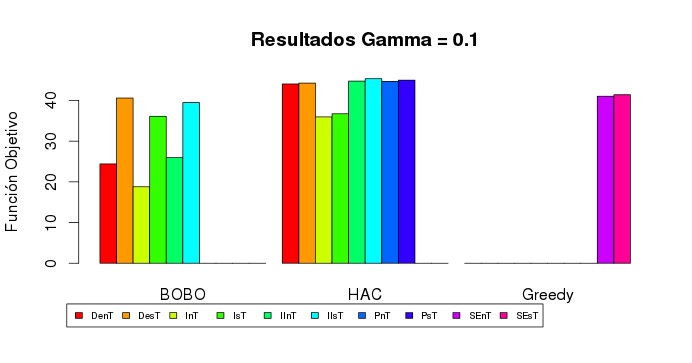
\includegraphics[width=0.8\textwidth]{resultados/papers/Graficos_agrupados/gamma01.png}
  \caption{Función Objetivo $\gamma$ = $0.1$ vs Algoritmos de resolución}
  \label{res:img-papers-agr-gamma01}
\end{figure}

\begin{figure}[H]
  \centering
    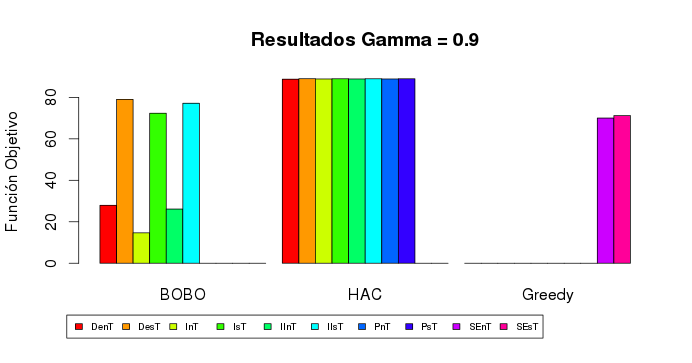
\includegraphics[width=0.8\textwidth]{resultados/papers/Graficos_agrupados/gamma09.png}
  \caption{Función Objetivo $\gamma$ = $0.9$ vs Algoritmos de resolución}
  \label{res:img-papers-agr-gamma09}
\end{figure}

De lo anterior se observa para todas las soluciones obtenidas, se puede mejorar la función objetivo aplicando la búsqueda tabú, aún sea en un valor pequeño. Otra observación interesante es que en todos los valores de $\gamma$ utilizados el algoritmo BOBO fue el más beneficiado en el uso de la búsqueda Tabú, sobre todo en las más altos. De forma inversa a lo que sucedía con los resultados iniciales que a medida que $\gamma$ crecía la función objetivo disminuía, utilizando la heurística revirtió la tendencia.\\
Para el HAC y la Búsqueda Golosa, el uso de Búsqueda Tabú tuvo un comportamiento similar entre las diferentes soluciones.\\

\paragraph{Jerarquico (o SingleHAC)}
En \ref{res:img-papers-agr-gamma01} y \ref{res:img-papers-agr-gamma09} se visualiza que utilizando una búsqueda Tabú al final de la ejecución  de HAC no mejora considerablemente la solución. Por lo que se decidió para este caso comparar el algoritmo sin la búsqueda tabú.
\begin{figure}[H]
  \centering
    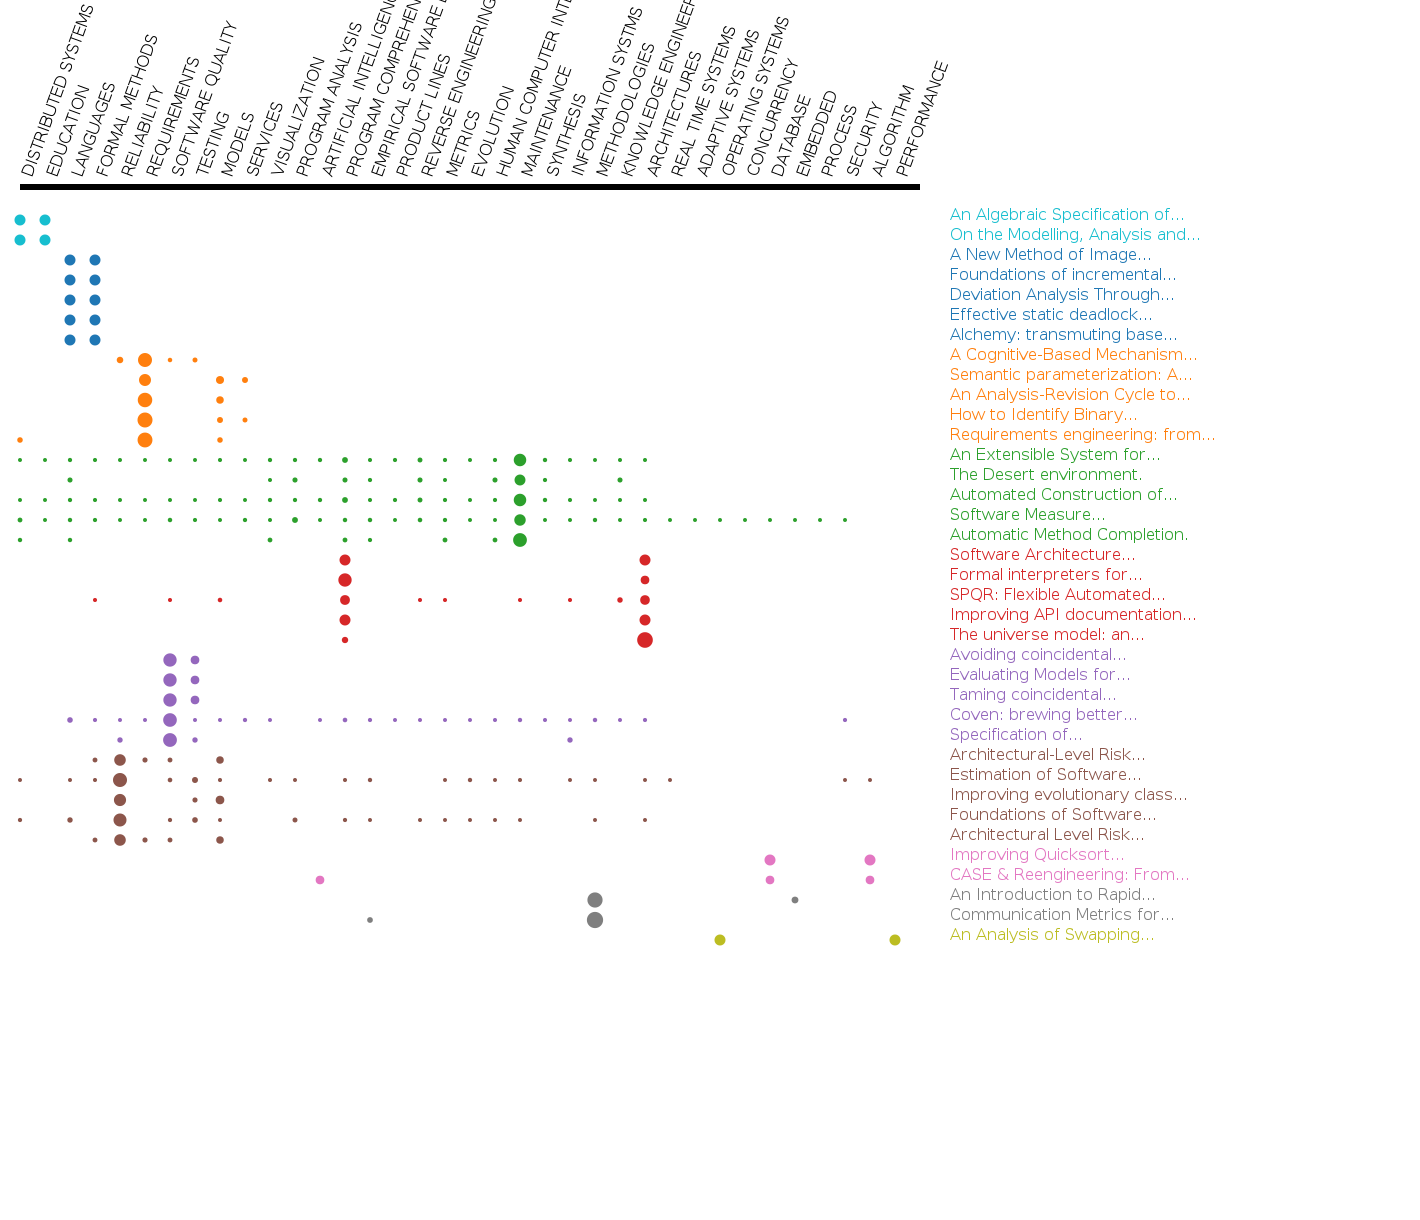
\includegraphics[width=0.8\textwidth]{resultados/papers/HAC/INTRA_INTER/gamma-01.png}
  \caption{Distribución de los perfiles por paper y bundle $\gamma$ = $0.1$ y HAC - Intra Inter}
  \label{res:img-papers-gamma01-hac-intra-inter}
\end{figure}

\begin{figure}[H]
  \centering
    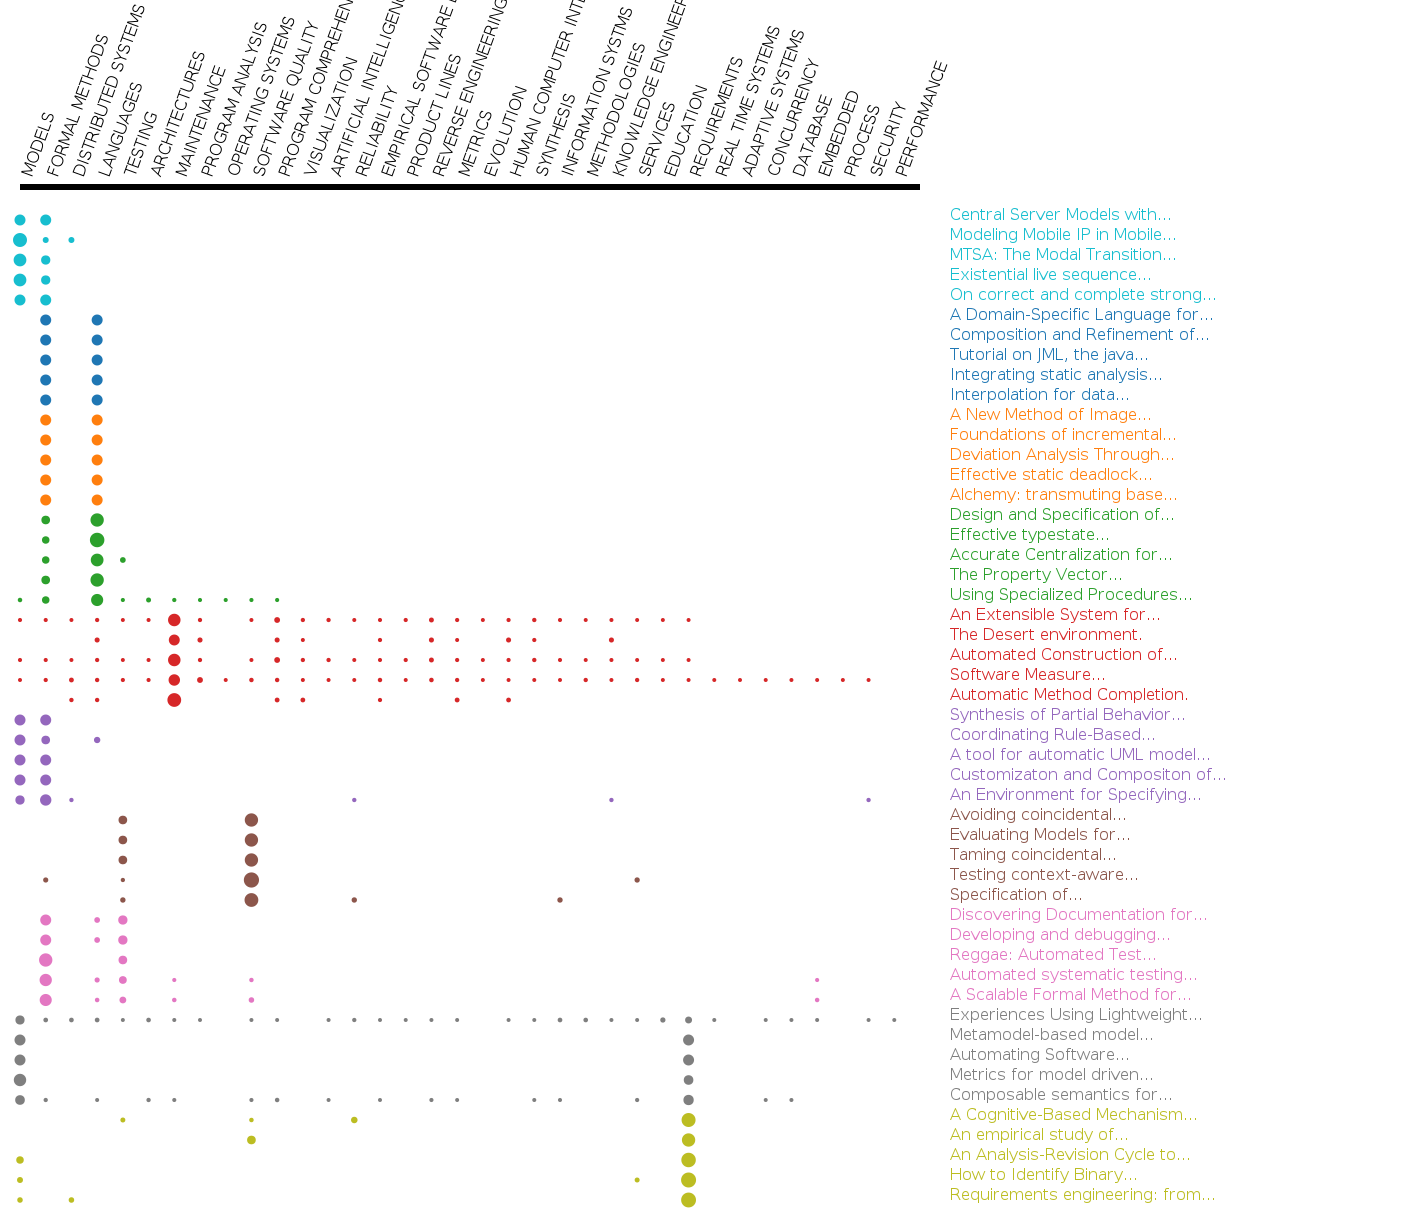
\includegraphics[width=0.8\textwidth]{resultados/papers/HAC/INTRA_INTER/gamma-09.png}
  \caption{Distribución de los perfiles por paper y bundle $\gamma$ = $0.9$ y HAC - Intra Inter}
  \label{res:img-papers-gamma09-hac-intra-inter}
\end{figure}

\begin{figure}[H]
  \centering
    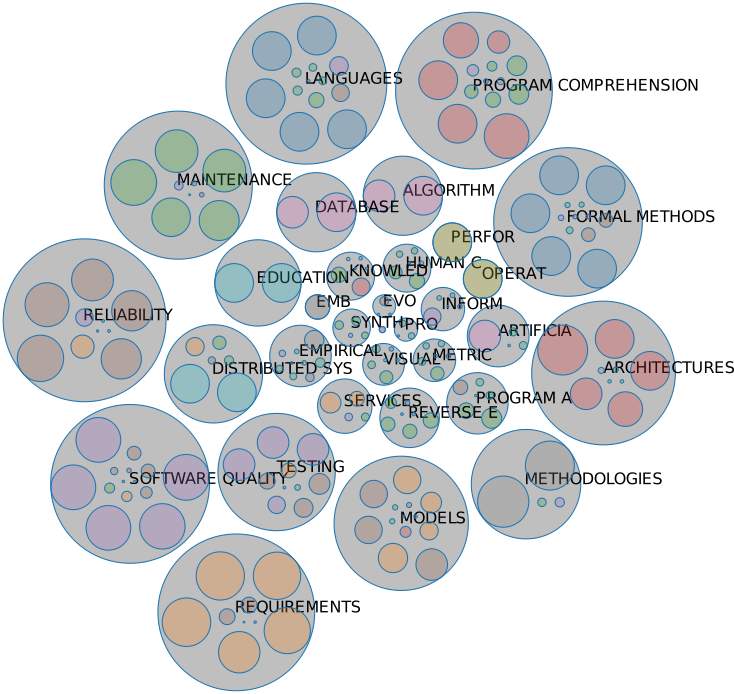
\includegraphics[width=0.8\textwidth]{resultados/papers/HAC/INTRA_INTER/bubbles-gamma-01.png}
  \caption{Distribución de los papers por perfil $\gamma$ = $0.1$ y HAC - Intra Inter}
  \label{res:img-papers-bubbles-gamma01-hac-intra-inter}
\end{figure}

\begin{figure}[H]
  \centering
    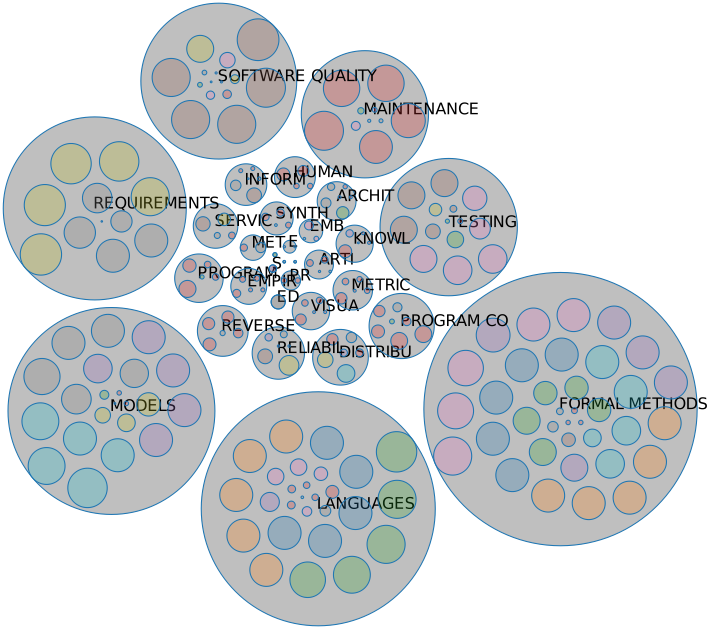
\includegraphics[width=0.8\textwidth]{resultados/papers/HAC/INTRA_INTER/bubbles-gamma-09.png}
  \caption{Distribución de los papers por perfil $\gamma$ = $0.9$ y HAC - Intra Inter}
  \label{res:img-papers-bubbles-gamma09-hac-intra-inter}
\end{figure}

De los gráficos \ref{res:img-papers-gamma01-hac-intra-inter} y \ref{res:img-papers-gamma09-hac-intra-inter} se puede observar como para $\gamma$ de valor bajo los perfiles de los artículos elegidos se encuentran más distribuidos entre los tópicos mientras que para valores más altos el mayor porcentaje se concentra en un pocos perfiles, generando en este último bundles más cohesivos como se está buscando, pero a la vez se tiene menos diversidad ya que en toda la solución se concentran los valores más representantivos de los perfiles de los artículos en un pocos como bien puede observarse en \ref{res:img-papers-bubbles-gamma09-hac-intra-inter}.\\
El comportamiento fue el mismo para todas las estrategias de selección que se utilizaron, la única diferencia fueron los valores finales de la función objetivo.
\paragraph{BOBO-100}
En este caso al ser muy grande la diferencia entre entre la utilización de la heurística Tabú y la ejecución sin ella,  se incluyó para poder visualizar los cambios en la solución.
\begin{figure}[H]
  \centering
    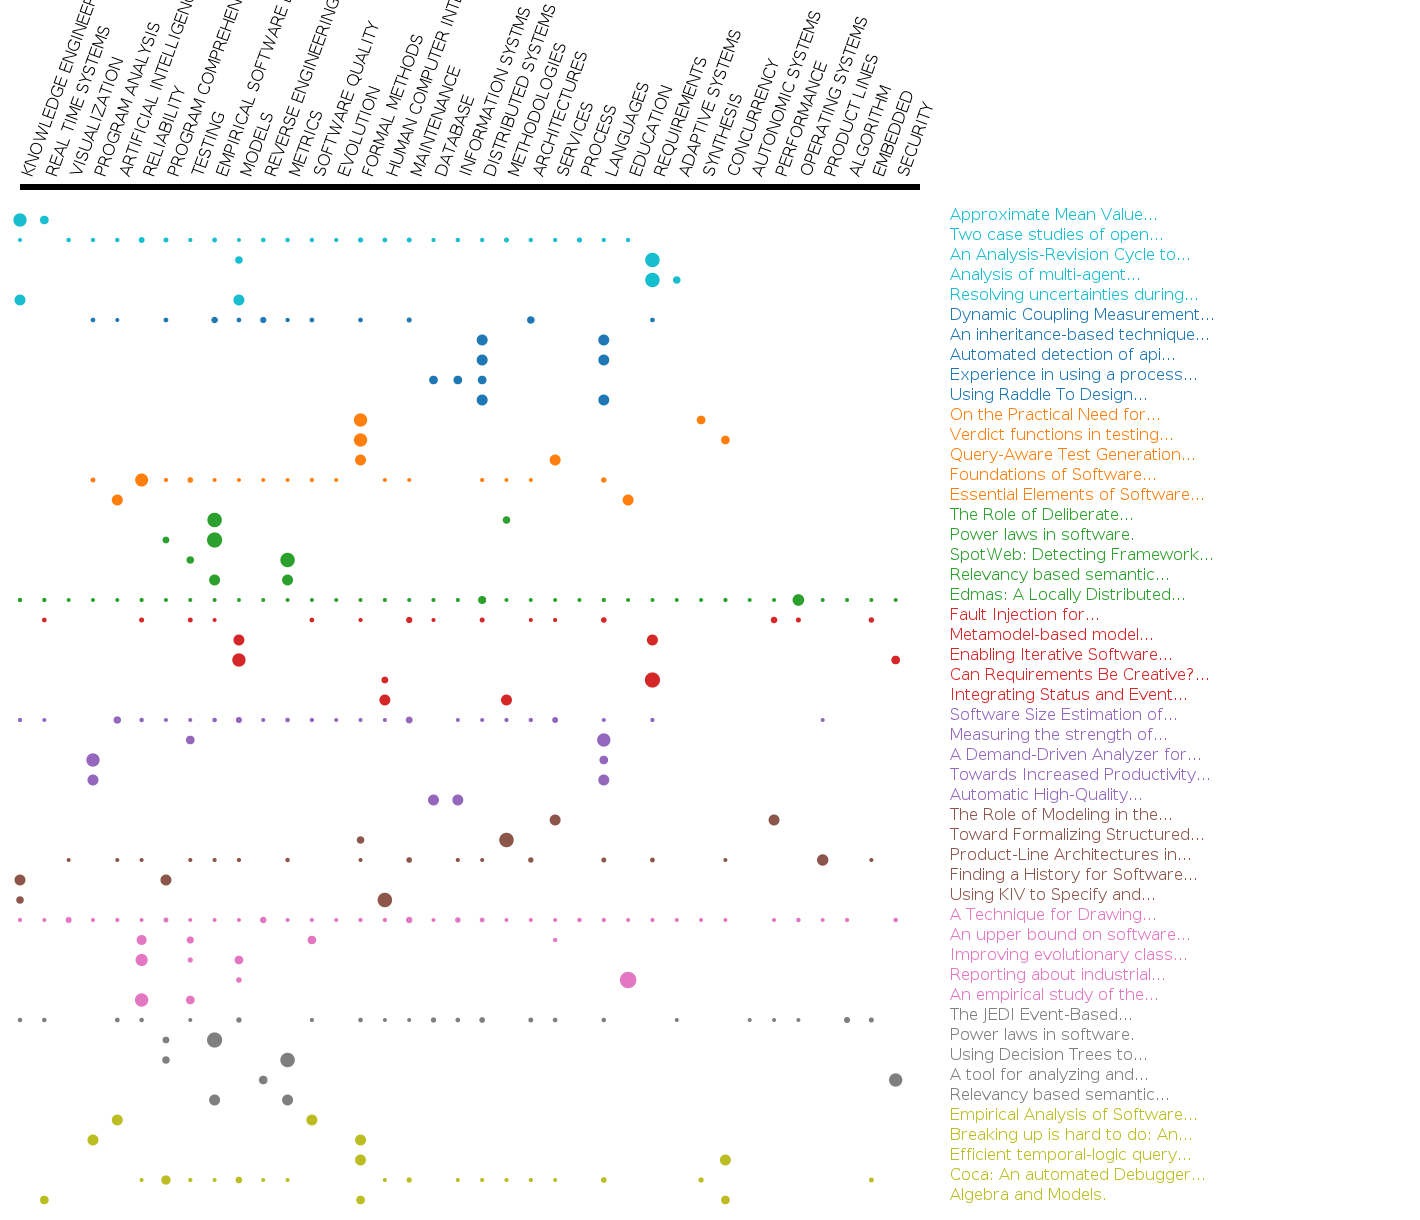
\includegraphics[width=0.8\textwidth]{resultados/papers/BOBO/INTRA_INTER/gamma-01.png}
  \caption{Distribución de los perfiles por paper y bundle $\gamma$ = $0.1$ y BOBO - Intra Inter}
  \label{res:img-papers-gamma01-bobo-intra-inter}
\end{figure}

\begin{figure}[H]
  \centering
    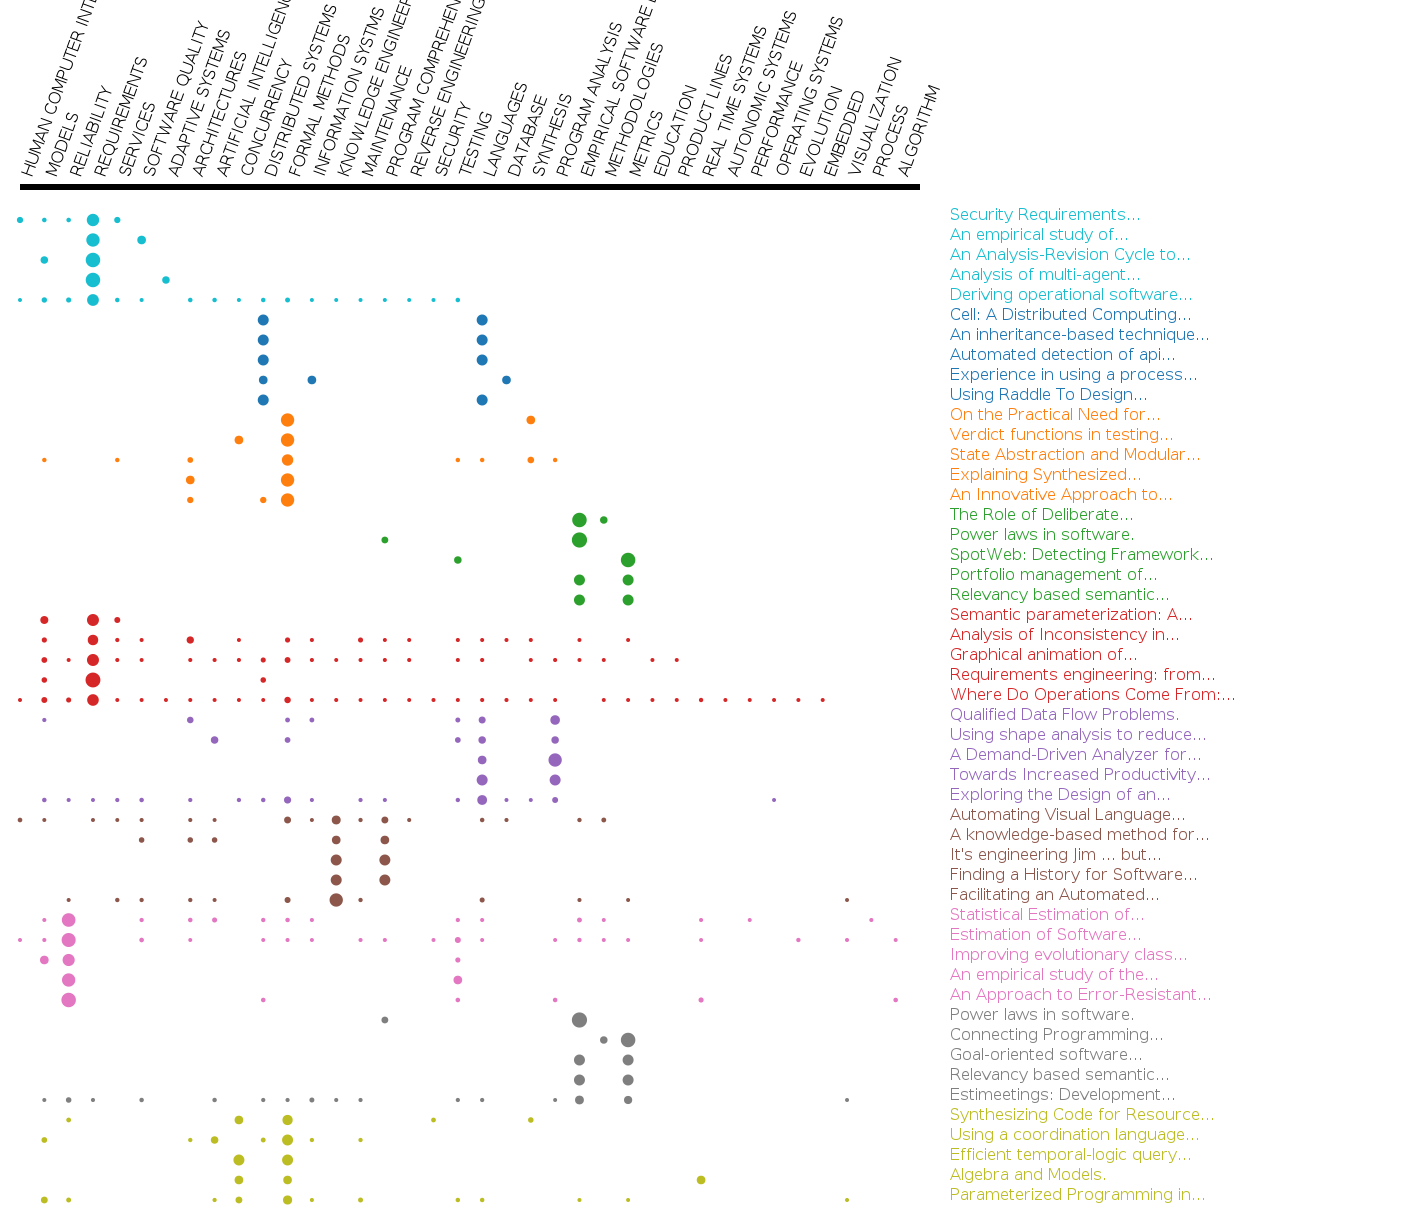
\includegraphics[width=0.8\textwidth]{resultados/papers/BOBO/INTRA_INTER/gamma-with-local-01.png}
  \caption{Distribución de los perfiles por paper y bundle $\gamma$ = $0.1$ y BOBO - Intra Inter con búsqueda Tabú}
  \label{res:img-papers-gamma01-bobo-intra-inter-tabu}
\end{figure}

\begin{figure}[H]
  \centering
    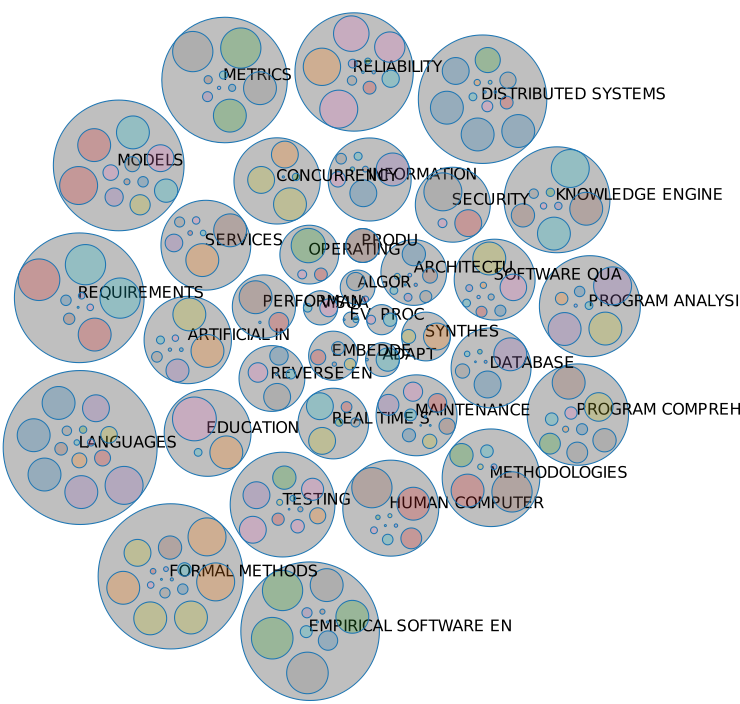
\includegraphics[width=0.8\textwidth]{resultados/papers/BOBO/INTRA_INTER/bubbles-gamma-01.png}
  \caption{Distribución de los papers por perfil $\gamma$ = $0.1$ y BOBO - Intra Inter}
  \label{res:img-papers-bubbles-gamma01-bobo-intra-inter}
\end{figure}

\begin{figure}[H]
  \centering
    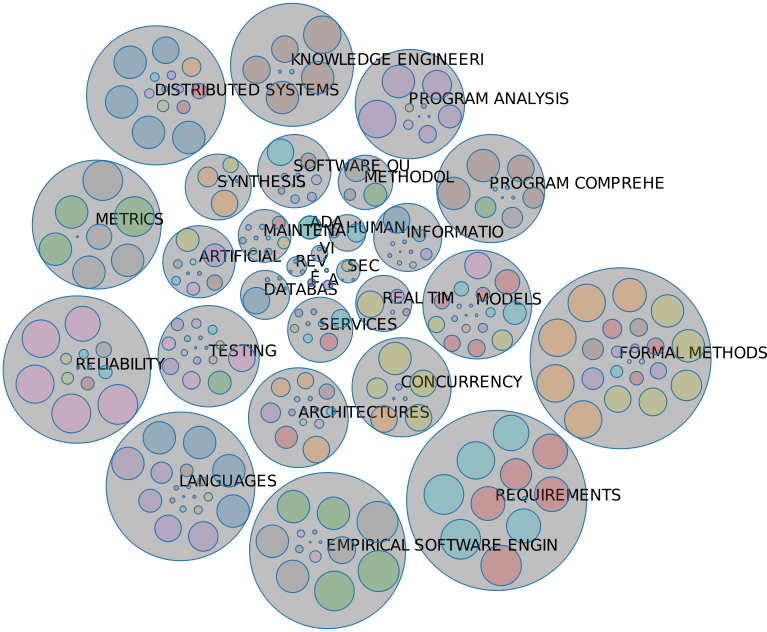
\includegraphics[width=0.8\textwidth]{resultados/papers/BOBO/INTRA_INTER/bubbles-gamma-with-local-01.png}
  \caption{Distribución de los papers por perfil $\gamma$ = $0.1$ y BOBO - Intra Inter con búsqueda Tabú}
  \label{res:img-papers-bubbles-gamma01-hac-intra-inter-bobo}
\end{figure}

\begin{figure}[H]
  \centering
    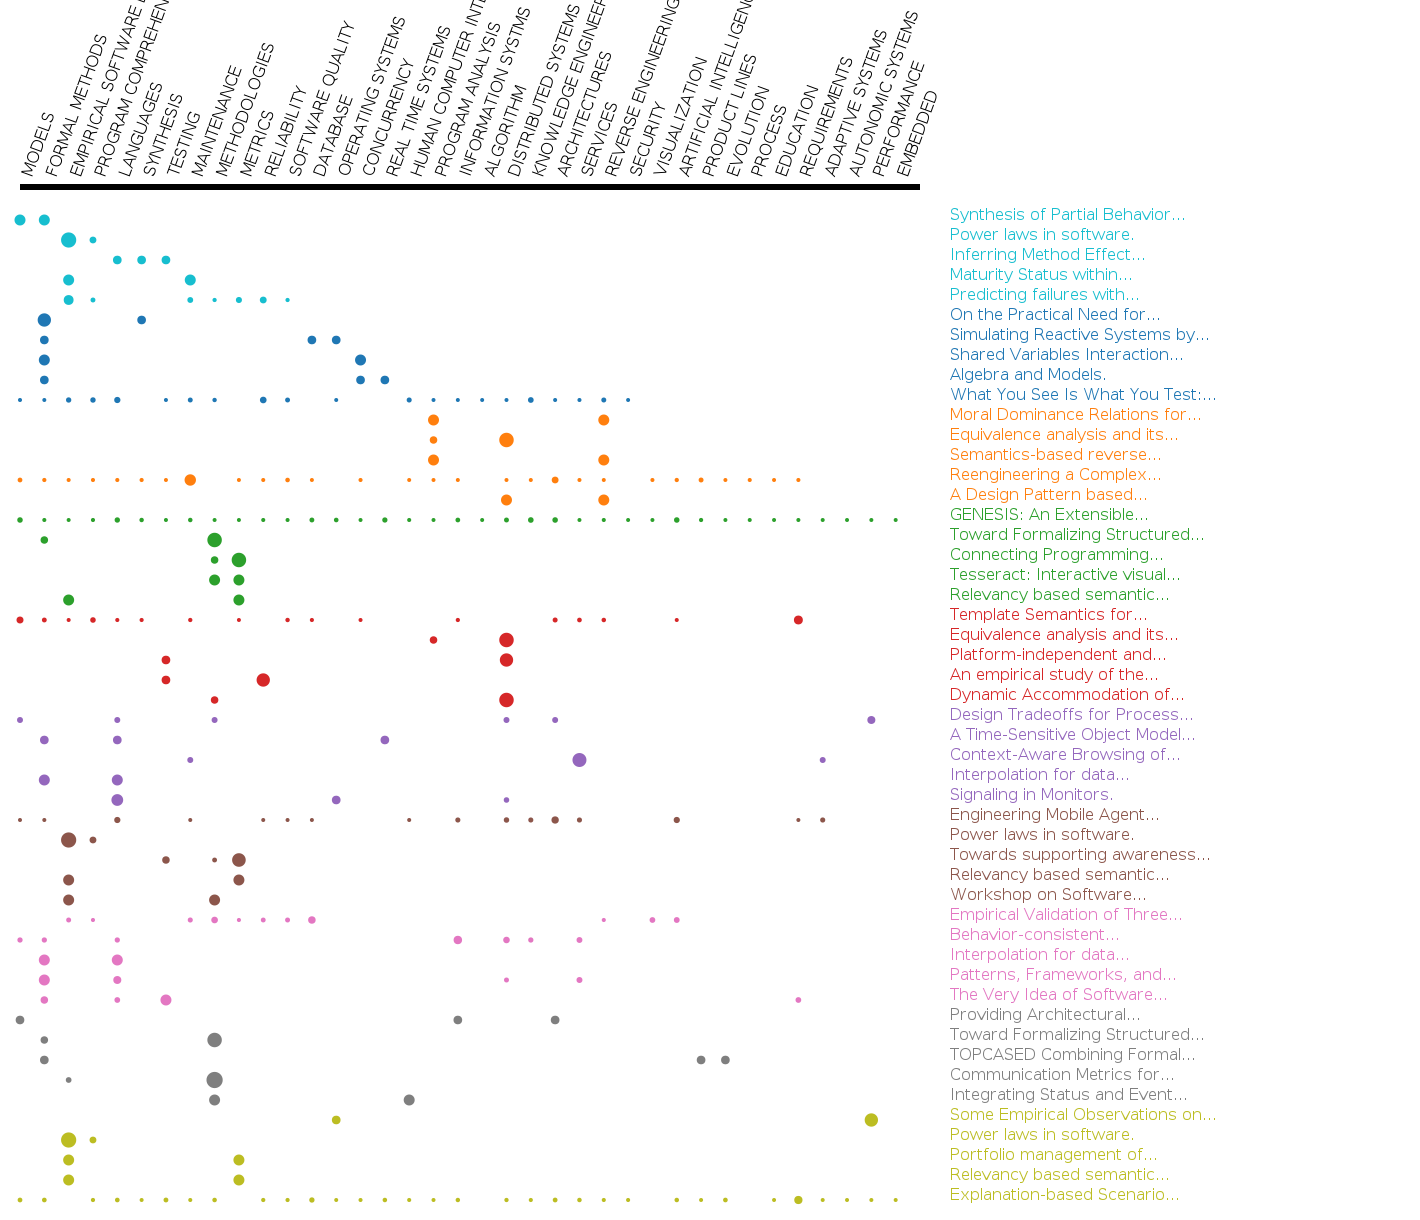
\includegraphics[width=0.8\textwidth]{resultados/papers/BOBO/INTRA_INTER/gamma-09.png}
  \caption{Distribución de los perfiles por paper y bundle $\gamma$ = $0.9$ y BOBO - Intra Inter}
  \label{res:img-papers-gamma09-bobo-intra-inter}
\end{figure}

\begin{figure}[H]
  \centering
    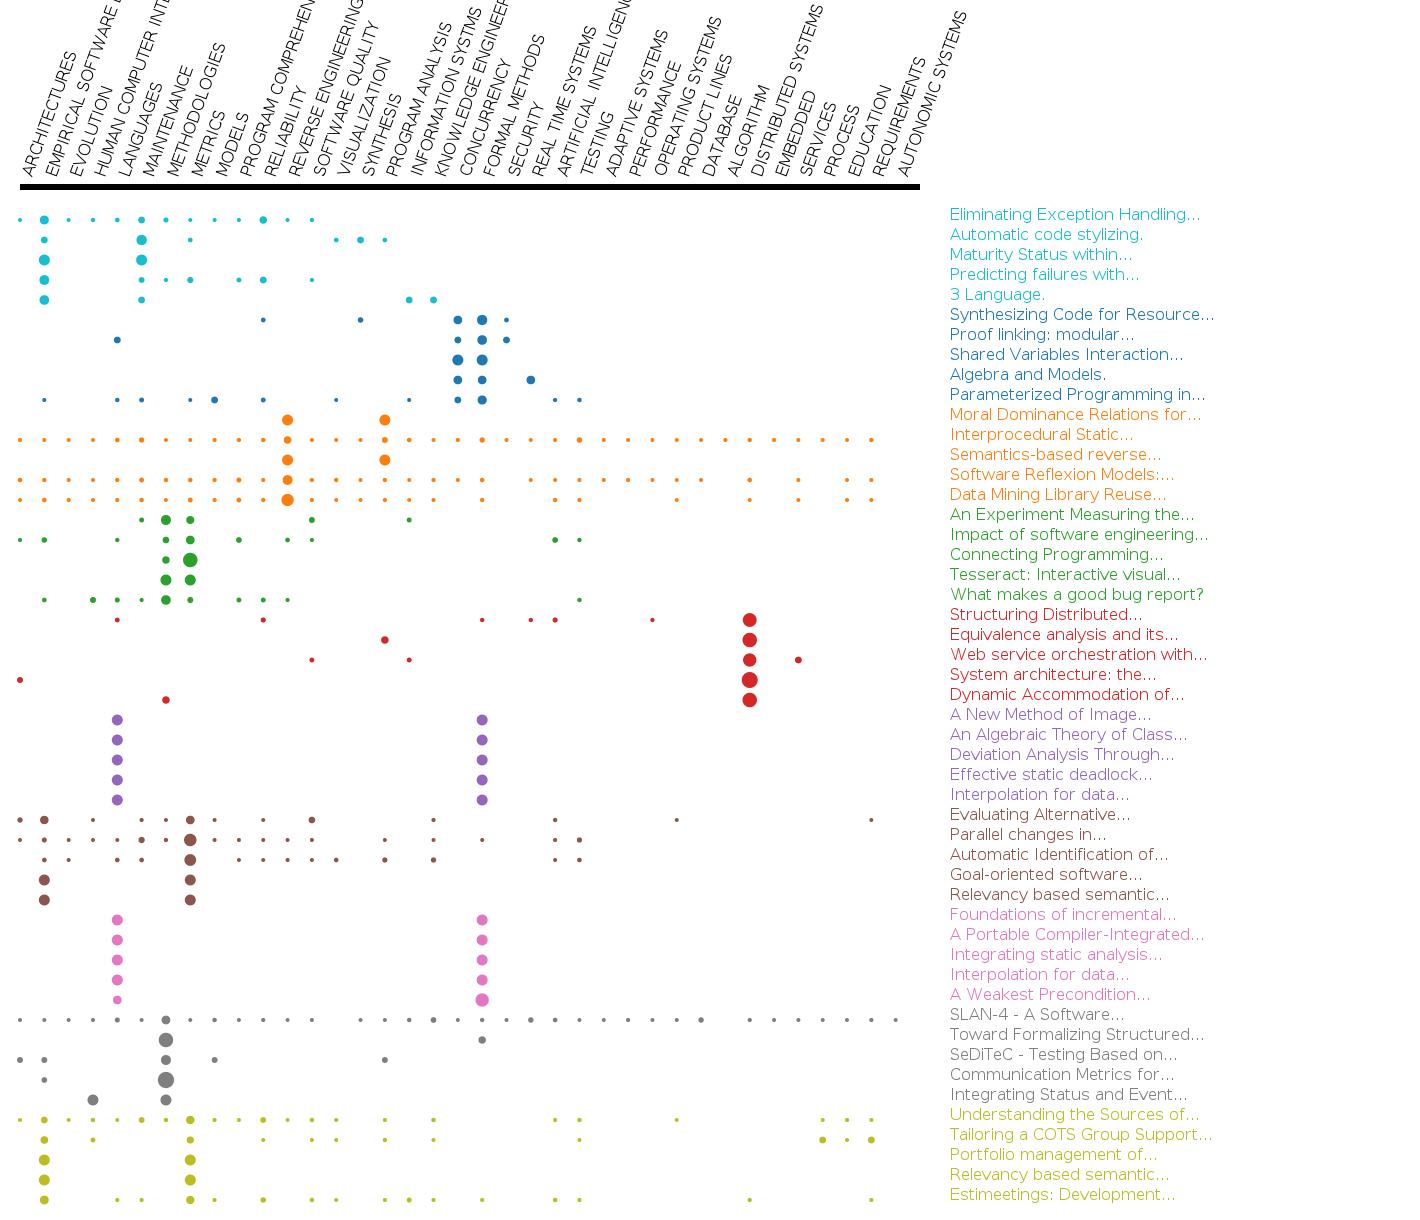
\includegraphics[width=0.8\textwidth]{resultados/papers/BOBO/INTRA_INTER/gamma-with-local-09.png}
  \caption{Distribución de los perfiles por paper y bundle $\gamma$ = $0.9$ y BOBO - Intra Inter con búsqueda Tabú}
  \label{res:img-papers-gamma09-bobo-intra-inter-tabu}
\end{figure}

\begin{figure}[H]
  \centering
    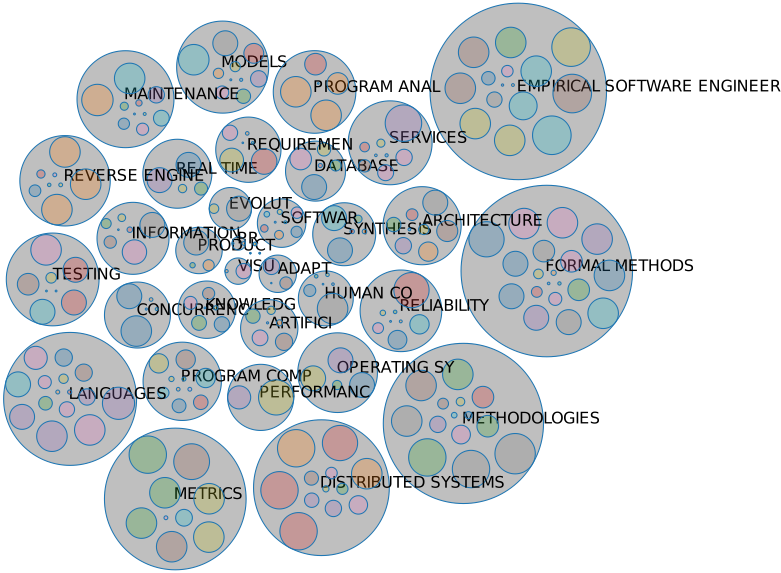
\includegraphics[width=0.8\textwidth]{resultados/papers/BOBO/INTRA_INTER/bubbles-gamma-09.png}
  \caption{Distribución de los papers por perfil $\gamma$ = $0.9$ y BOBO - Intra Inter}
  \label{res:img-papers-bubbles-gamma09-bobo-intra-inter}
\end{figure}

\begin{figure}[H]
  \centering
    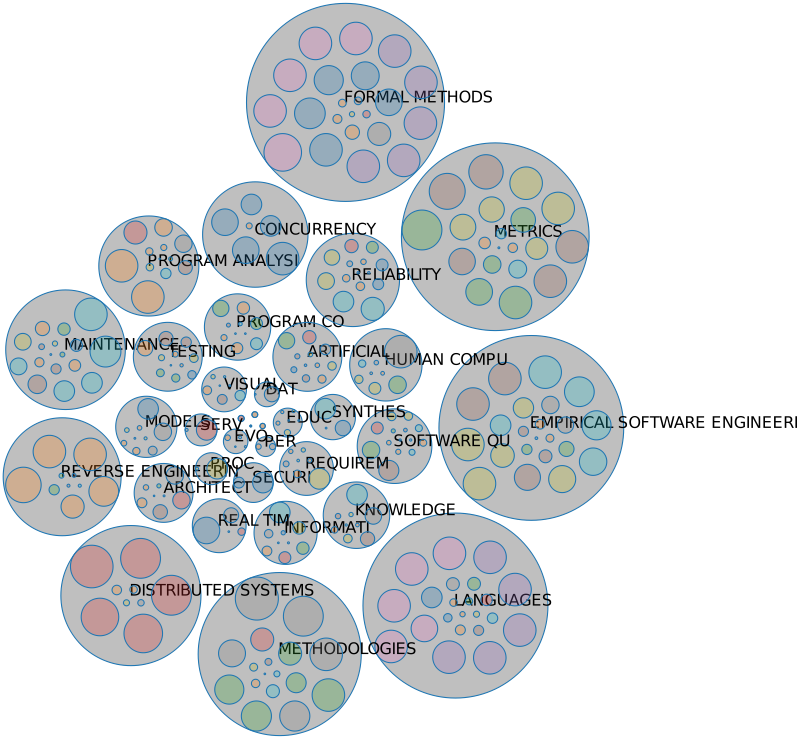
\includegraphics[width=0.8\textwidth]{resultados/papers/BOBO/INTRA_INTER/bubbles-gamma-with-local-09.png}
  \caption{Distribución de los papers por perfil $\gamma$ = $0.9$ y BOBO - Intra Inter con búsqueda Tabú}
  \label{res:img-papers-bubbles-gamma09-hac-intra-inter-bobo}
\end{figure}
\newpage
\subsection{Búsqueda de Autores}
Solución de bundles en el que cada uno contiene autores similares de distinta universidad de afiliación.\\
\begin{itemize}
  \item \textbf{Similitud}: Función que compara el perfil de los autores.
  \item \textbf{Complementariedad}: Universidad de pertenencia del autor.
\end{itemize}

La instancia elegida, luego de la depuración mencionada en \ref{res:busPaper}, cuenta con $5577$ autores en condiciones de ser elegidos por los algoritmos implementados.\\
Al igual que con las búsquedas de artículos se realizaron las mismas ejecuciones con los mismos parámetros, es decir, se generaron soluciones con las siguientes características:\\
\Solucion
{}
{\texttt{SingleHAC}, \texttt{Búsqueda Golosa} y \texttt{BOBO-100}}
{Denset Subgraph, Intra, Intra-Inter, Proportional (no aplican a la búsqueda golosa)}
{$\in$ $(0,1; 0,3; 0,5; 0,7; 0,9)$}
{10}
{5}

\begin{figure}[H]
  \centering
    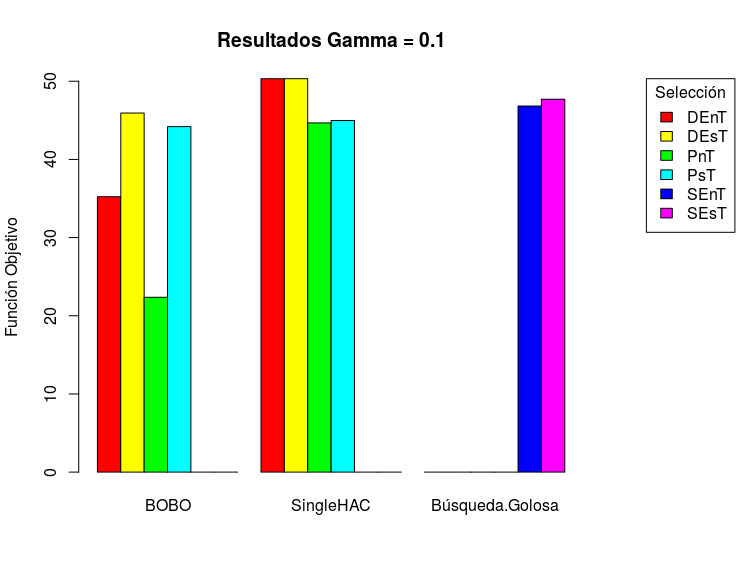
\includegraphics[width=0.8\textwidth]{resultados/authors/Graficos_agrupados/gamma01-autores.png}
  \caption{Función Objetivo $\gamma$ = $0.1$ vs Algoritmos de resolución}
  \label{res:img-autores-agr-gamma01}
\end{figure}

\begin{figure}[H]
  \centering
    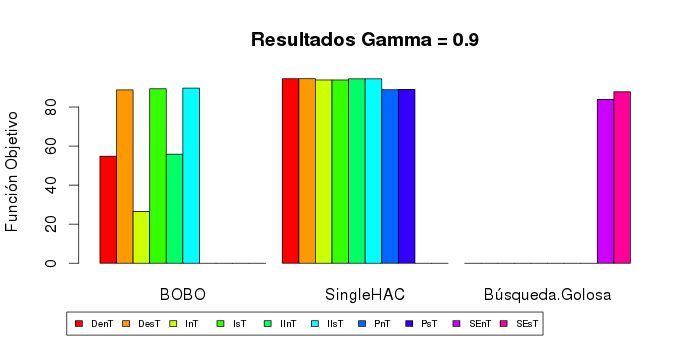
\includegraphics[width=0.8\textwidth]{resultados/authors/Graficos_agrupados/gamma09-autores.png}
  \caption{Función Objetivo $\gamma$ = $0.9$ vs Algoritmos de resolución}
  \label{res:img-autores-agr-gamma09}
\end{figure}

El comportamiento de las ejecuciones fueron muy similares a las que se obtuvieron en la búsqueda de artículos, la utilización de la Búsqueda Tabú mejoró sustancialmente el algoritmo \texttt{BOBO} en todos sus variantes. En el caso de \texttt{SingleHAC}, solo mejoró con la estratégia de selección \texttt{Proportional}. Casualmente fue la única estratégia que tuvo un comportamiento diferente en relación a la búsqueda de artículos, en la cuál su función objetivo siempre tuvo valores mayores o iguales a por ejemplo la selección \texttt{INTRA} y en este caso fue menor o igual. Igualmente las difrencias en términos de valor son mínimas y se deben a la conformación de los perfiles de los elementos.\\
Como se menciona anteriormente, al no comportarse de una manera diferente a la búsqueda de artículos no se incluyeron los gráficos.
\section{Atracciones turísticas}\label{res:busAtracciones}
Aquí se muestran las soluciones en las que cada bundle representa un conjunto de atracciones que un turista puede visitar, cada uno de ellos no supera el presupuesto máximo y cada elemento es un tipo de atracción diferente.
\begin{itemize}
  \item \textbf{Similitud}: Los valores fueron entregados ya calculados.
  \item \textbf{Complementariedad}: Tipo de atracción turística.
  \item \textbf{presupuesto}: Valor de la atracción.
\end{itemize}
Se generaron soluciones con las siguientes características:\\
\SolucionBudget
{}
{\texttt{SingleHAC}, \texttt{Búsqueda Golosa} y \texttt{BOBO-100}}
{Intra-Inter, Proportional (no aplica a la búsqueda golosa)}
{$\in$ $(0,1; 0,3; 0,5; 0,7; 0,9)$}
{10}
{3}
{7}

\begin{figure}[H]
  \centering
    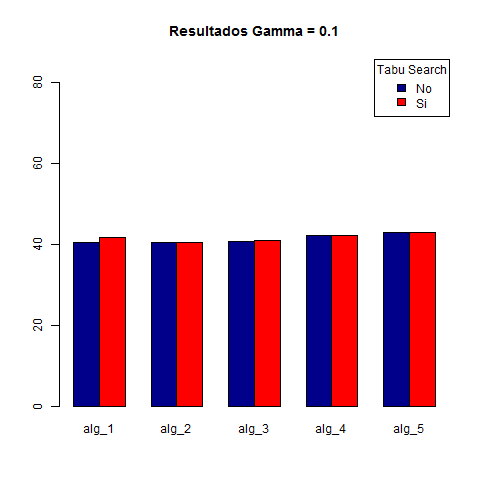
\includegraphics[width=0.8\textwidth]{resultados/cities/Graficos_agrupados/gamma01-cities.png}
  \caption{Función Objetivo $\gamma$ = $0.1$ vs Algoritmos de resolución}
  \label{res:img-cities-agr-gamma01}
\end{figure}

\begin{figure}[H]
  \centering
    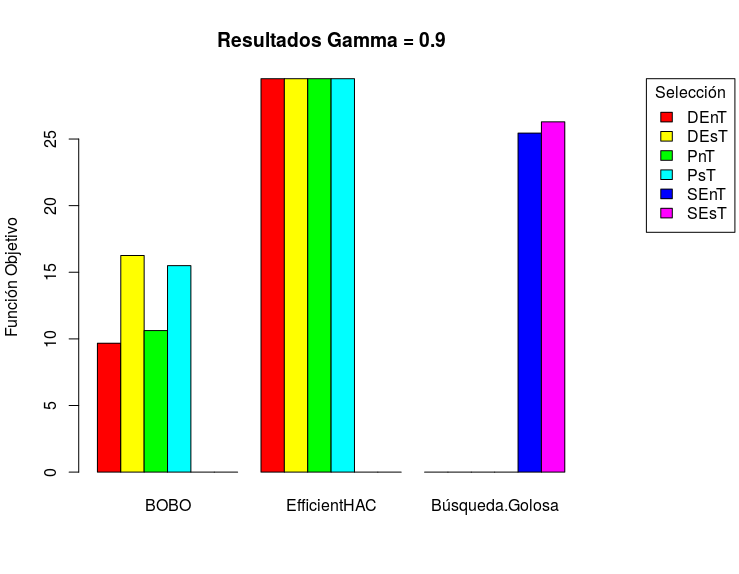
\includegraphics[width=0.8\textwidth]{resultados/cities/Graficos_agrupados/gamma09-cities.png}
  \caption{Función Objetivo $\gamma$ = $0.9$ vs Algoritmos de resolución}
  \label{res:img-cities-agr-gamma09}
\end{figure}

Al igual que en los demas escenarios de ejecuciones el comportamiento fue el esperado y en todas las estrategias usadas para los distintos algoritmos, aplicando la búsqueda Tabú a la solución obtenida encuentra siempre una mejor. También se puede observar que usando la implementación BOBO para valores de $\gamma$ altos es donde mejor funciona la metaheurística y que la búsqueda golosa siempre esta debajo de la solución HAC.\\
Solo se muestran los gráficos y comportamientos para las pruebas realizadas con un solo presupuesto, pero los mismos tuvieron el mismo efecto a medida que se cambiaba el valor.